%% abtex2-modelo-artigo.tex, v-1.9.7 laurocesar
%% Copyright 2012-2018 by abnTeX2 group at http://www.abntex.net.br/ 
%%
%% This work may be distributed and/or modified under the
%% conditions of the LaTeX Project Public License, either version 1.3
%% of this license or (at your option) any later version.
%% The latest version of this license is in
%%   http://www.latex-project.org/lppl.txt
%% and version 1.3 or later is part of all distributions of LaTeX
%% version 2005/12/01 or later.
%%
%% This work has the LPPL maintenance status `maintained'.
%% 
%% The Current Maintainer of this work is the abnTeX2 team, led
%% by Lauro César Araujo. Further information are available on 
%% http://www.abntex.net.br/
%%
%% This work consists of the files abntex2-modelo-artigo.tex and
%% abntex2-modelo-references.bib
%%

% ------------------------------------------------------------------------
% ------------------------------------------------------------------------
% abnTeX2: Modelo de Artigo Acadêmico em conformidade com
% ABNT NBR 6022:2018: Informação e documentação - Artigo em publicação 
% periódica científica - Apresentação
% ------------------------------------------------------------------------
% ------------------------------------------------------------------------

\documentclass[
	% -- opções da classe memoir --
	article,			% indica que é um artigo acadêmico
	11pt,				% tamanho da fonte
	oneside,			% para impressão apenas no recto. Oposto a twoside
	a4paper,			% tamanho do papel. 
	% -- opções da classe abntex2 --
	%chapter=TITLE,		% títulos de capítulos convertidos em letras maiúsculas
	%section=TITLE,		% títulos de seções convertidos em letras maiúsculas
	%subsection=TITLE,	% títulos de subseções convertidos em letras maiúsculas
	%subsubsection=TITLE % títulos de subsubseções convertidos em letras maiúsculas
	% -- opções do pacote babel --
	english,			% idioma adicional para hifenização
	brazil,				% o último idioma é o principal do documento
	sumario=tradicional
	]{abntex2}


% ---
% PACOTES
% ---

% ---
% Pacotes fundamentais 
% ---
\usepackage{lmodern}			% Usa a fonte Latin Modern
\usepackage[T1]{fontenc}		% Selecao de codigos de fonte.
\usepackage[utf8]{inputenc}		% Codificacao do documento (conversão automática dos acentos)
\usepackage{indentfirst}		% Indenta o primeiro parágrafo de cada seção.
\usepackage{nomencl} 			% Lista de simbolos
\usepackage{color}				% Controle das cores
\usepackage{graphicx}			% Inclusão de gráficos
\usepackage{microtype} 			% para melhorias de justificação
\usepackage[]{algorithm2e}
% ---
		
% ---
% Pacotes adicionais, usados apenas no âmbito do Modelo Canônico do abnteX2
% ---
\usepackage{lipsum}				% para geração de dummy text
% ---
		
% ---
% Pacotes de citações
% ---
\usepackage[brazilian,hyperpageref]{backref}	 % Paginas com as citações na bibl
\usepackage[alf]{abntex2cite}	% Citações padrão ABNT
% ---

% ---
% Configurações do pacote backref
% Usado sem a opção hyperpageref de backref
\renewcommand{\backrefpagesname}{Citado na(s) página(s):~}
% Texto padrão antes do número das páginas
\renewcommand{\backref}{}
% Define os textos da citação
\renewcommand*{\backrefalt}[4]{
	\ifcase #1 %
		Nenhuma citação no texto.%
	\or
		Citado na página #2.%
	\else
		Citado #1 vezes nas páginas #2.%
	\fi}%
% ---

% --- Informações de dados para CAPA e FOLHA DE ROSTO ---
\titulo{Proposta de solução do Problema de Dominação de Rainhas Utilizando ILS}
\tituloestrangeiro{Proposed solution to the Minimum Dominating Set of Queens Problem using ILS}


\autor{Maria Edoarda Vallim Fonseca \and Thales Athayde Santos}
%\email{medoarda@id.uff.br}
%\email{thalesathaydesantos@id.uff.br}

\local{Brasil}
\data{2018, v-1.0.0}
% ---

% ---
% Configurações de aparência do PDF final

% alterando o aspecto da cor azul
\definecolor{blue}{RGB}{41,5,195}

% informações do PDF
\makeatletter
\hypersetup{
     	%pagebackref=true,
		pdftitle={\@title}, 
		pdfauthor={\@author},
    	pdfsubject={Proposta de solução do Problema de Dominação de Rainhas Utilizando ILS},
	    pdfcreator={LaTeX with abnTeX2},
		pdfkeywords={ILS}{Algoritmo Genético}{Problema de Dominação de Rainhas}, 
		colorlinks=true,       		% false: boxed links; true: colored links
    	linkcolor=blue,          	% color of internal links
    	citecolor=blue,        		% color of links to bibliography
    	filecolor=magenta,      		% color of file links
		urlcolor=blue,
		bookmarksdepth=4
}
\makeatother
% --- 

% ---
% compila o indice
% ---
\makeindex
% ---

% ---
% Altera as margens padrões
% ---
\setlrmarginsandblock{3cm}{3cm}{*}
\setulmarginsandblock{3cm}{3cm}{*}
\checkandfixthelayout
% ---

% --- 
% Espaçamentos entre linhas e parágrafos 
% --- 

% O tamanho do parágrafo é dado por:
\setlength{\parindent}{1.3cm}

% Controle do espaçamento entre um parágrafo e outro:
\setlength{\parskip}{0.2cm}  % tente também \onelineskip

% Espaçamento simples
\SingleSpacing


% ----
% Início do documento
% ----
\begin{document}

% Seleciona o idioma do documento (conforme pacotes do babel)
%\selectlanguage{english}
\selectlanguage{brazil}

% Retira espaço extra obsoleto entre as frases.
\frenchspacing 

% ----------------------------------------------------------
% ELEMENTOS PRÉ-TEXTUAIS
% ----------------------------------------------------------

%---
%
% Se desejar escrever o artigo em duas colunas, descomente a linha abaixo
% e a linha com o texto ``FIM DE ARTIGO EM DUAS COLUNAS''.
% \twocolumn[    		% INICIO DE ARTIGO EM DUAS COLUNAS
%
%---

% página de titulo principal (obrigatório)
\maketitle


% titulo em outro idioma (opcional)



% resumo em português
\begin{resumoumacoluna}
Neste artigo, propomos uma solução para o Problema de Dominação de Rainhas usando Busca Iterativa Local e comparamos nossos resultados com uma solução prévia utilizando Algoritmo Genético.
 
 \vspace{\onelineskip}
 
 \noindent
 \textbf{Palavras-chave}: Problema de Dominação de Rainhas. Busca Iterativa Local. Metaheurística.
\end{resumoumacoluna}


% resumo em inglês
\renewcommand{\resumoname}{Abstract}
\begin{resumoumacoluna}
 \begin{otherlanguage*}{english}
  In this paper, we propose a solution to the Dominating Set of Queens Problem
  using Iterative Local Search and compare our results with a previous 
  solution using Genetic Algorithm.

   \vspace{\onelineskip}
 
   \noindent
   \textbf{Keywords}: Dominating Queen Problem. ILS. Metaheuristic.
 \end{otherlanguage*}  
\end{resumoumacoluna}

% ]  				% FIM DE ARTIGO EM DUAS COLUNAS
% ---

\begin{center}\smaller
\textbf{Data de submissão e aprovação}: elemento obrigatório. Indicar dia, mês e ano

\textbf{Identificação e disponibilidade}: elemento opcional. Pode ser indicado 
o endereço eletrônico, DOI, suportes e outras informações relativas ao acesso.
\end{center}

% ----------------------------------------------------------
% ELEMENTOS TEXTUAIS
% ----------------------------------------------------------
\textual

% ----------------------------------------------------------
% Introdução
% ----------------------------------------------------------
\section{Introdução}

O problema de dominação de rainhas é muito bem conhecido dentre os problemas de xadrez. Nele, dado um tabuleiro \textit{n $\times$ n}, temos n quadrados dispostos nas linhas e n quadrados nas colunas. Quando uma rainha Q é disposta no tabuleiro, ela domina a linha, a coluna, e as diagonais que passam pela sua posição.~\ref{fig:1rainha} O objetivo do problema é descobrir a disposição da menor quantidade de rainhas possível de forma à dominar todo o tabuleiro.

 Algoritmos evolucionários provaram ter sucesso para resolver e otimizar uma grande variedade de problemas complexos, incluindo problemas combinatórios, como o estudado aqui, em um tempo computacional razoavelmente aceitável.~\cite{doerr2011evolutionary}

\textit{Local Search}, ou Busca Local, é um método heurístico para resolver problemas computacionalmente difíceis. Busca local pode ser usada em problemas que possam ser formulados como achar a solução maximizando um critério entre várias soluções possíveis. Algoritmos de busca local movem de solução à solução no espaço de soluções possíveis aplicando mudanças locais, até uma solução dita ótima ser encontrada.~\cite{hoos2004stochastic}

Um dos problemas da Busca Local é que ela pode ficar presa em um mínimo local, sem conseguir melhorar seu resultado. Para contornar esse problema, utiliza-se \textit{Iterative Local Search}, ou Busca Local Iterativa. Essa modificação consiste em iterar sobre chamadas da busca local, cada vez começando de um ponto diferente do conjunto de solução perturbando o mínimo local atual de modo que faça a solução chegar em outro ótimo local. Esta perturbação não pode ser muito forte nem muito fraca, pois corre o risco dela acabar encontrando o mesmo mínimo local ou servir como uma inicialização aleatória.~\cite{lourencco2010iterated}

  Neste artigo, propomos uma solução baseada em \textit{Iterative Local Search} para o Problema de Dominação de Rainhas. Nossos resultados serão comparados diretamente com o método descrito em~\cite{alharbi2017genetic}, que utiliza Algoritmo Genético e é o mais comumente encontrado para solucionar este problema. Depois disso, iremos debater os resultados alcançados.

  \begin{figure}
    \centering
    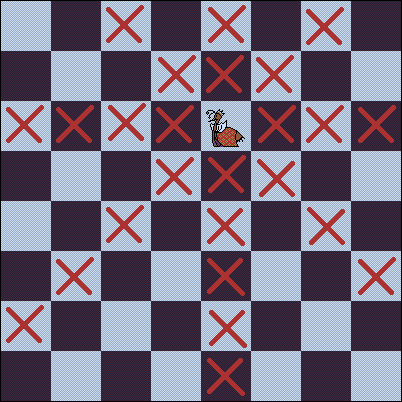
\includegraphics[width=0.60\linewidth]{dom1rainha8x8.png}
    \caption{Exemplo da linha de dominação de uma rainha em um tabuleiro de xadrez \textit{8 $\times$ 8}}
    \label{fig:1rainha}
  \end{figure}

% ----------------------------------------------------------
% Seção de explicações
% ----------------------------------------------------------
%%%%%%%%%%%%%%%%%%%%%%%%%%%%%%%%%%%%%%%%%%%%%%%%%%%%%%%%%%%%%%%%%%%%%%
\section{Motivação}

Decidimos escolher o \textit{Dominating Set of Queens Problem} por ter sido um dos temas abordados por um dos membros do grupo durante as apresentações de trabalho da disciplina, o que nos deu um certo grau de familiaridade com o assunto. Pesquisando mais à fundo, vimos que as soluções mais comuns para a solução do Problema de Dominação de Rainhas eram com \textit{Backtracking} e Algoritmo Genético. Além disso, de acordo com~\cite{alharbi2017genetic}, existem muitos artigos procurando os limites superior e inferior do problema, mas não existe muito esforço de pesquisa
na busca de soluções práticas para o problema.

Visto essa situação, decidimos propor uma solução baseada em \textit{Iterative Local Search} para o problema e comparar os resultados com uma solução em Algoritmo Guloso.

%%%%%%%%%%%%%%%%%%%%%%%%%%%%%%%%%%%%%%%%%%%%%%%%%%%%%%%%%%%%%%%%%%%%%%
\section{Trabalhos Relacionados}

\begin{figure}
  \centering
  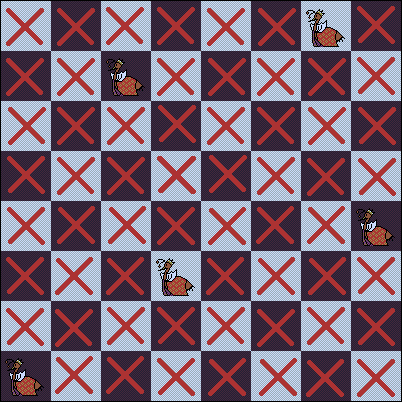
\includegraphics[width=0.60\linewidth]{dom2rainha8x8.png}
  \caption{Exemplo de um tabuleiro de tamanho \textit{8 $\times$ 8} sendo completamente dominado por
  quatro rainhas}
  \label{fig:2rainha}
\end{figure}

Um problema semelhante, proposto em 1850, conhecido como problema das n-rainhas teve muitos esforços focados nele para sua solução. O problema das n-rainhas é descrito como: dado um tabuleiro \textit{n $\times$ n}, qual seria a disposição das rainhas de modo que nenhuma rainha consiga atacar a outra. Houve muita pesquisa em torno deste problema, e suas soluções utilizam desde teoria matemática até teoria dos grafos. O estudo desse tipo de problema pode beneficiar várias áreas como controle de tráfego, prevenção de \textit{deadlocks} e armazenamento de memória paralela.~\cite{bell2009survey}

Muitas soluções para o problema das n rainhas foram propostas, dentre elas backtracking, redes neurais e algoritmos evolucionários.

Em contrapartida, o problema de dominação de rainhas não recebeu tanta atenção dentre os pesquisadores das ciências da computação. Na realidade, várias pesquisas se preocuparam em pesquisar o problema porém só adotaram modelos matemáticos.~\cite{alharbi2017genetic} Burger e Mynhart apontaram que o problema de dominação das rainhas é um dos mais difíceis problemas de xadrez.~\cite{art43}
Esse problema é comumente definido como achar o menor número possível de rainhas em um tabuleiro \textit{n $\times$ n} que consigam a dominação total do tabuleiro. Esse número é conhecido como número de dominação e sua notação é $\gamma(\textbf{Qn})$.
Muitos pesquisadores focaram em descobrir os limites superior e inferior do problema desde a década de 70,  e o número mínimo possível de rainhas para solucionar o problema ($\gamma(\textbf{Qn})$) foi calculado para diversos tamanhos de tabuleiro (vide tabela~\ref{tabela1})~\cite{art3,art43,art44,art45}.

\begin{table*}[ht]
  \caption{Número mínimo de rainhas para dominação total $\gamma(\textbf{Qn})$ de um tabuleiro de tamanho $\textit{n}$.}
  \begin{tabular}{l*{18}{c}r}
    n              & 1 & 2 & 3 & 4 & 5  & 6 & 7 & 8 & 9 & 10 & 11 & 12 & 13 & 14 & 15 & 16 & 17 & 18 \\
    \hline
    $\gamma(\textbf{Qn})$ & 1 & 1 & 1 & 3 & 3 & 4 & 4 & 5 & 5 & 5 & 5 & 7 & 7 & ~$\leq$8 & $\leq$9 & $\leq$9  & 9 & 9 \\
  \end{tabular}
  \label{tabela1}
\end{table*}

%%%%%%%%%%%%%%%%%%%%%%%%%%%%%%%%%%%%%%%%%%%%%%%%%%%%%%%%%%%%%%%%%%%%%%

\section{Formulação do Problema}

Para este problema ser usado num computador tivemos que fazer as seguintes coisas. 

Cada casa do tabuleiro é representada por uma tupla $(x,y)$ onde obviamente $x$ é o eixo \textit{x} e $y$ é o eixo \textit{y}. Com isso cada rainha é representada por um $(x,y)$ que é sua posição no tabuleiro.

Para representar um individuo a gente usa um conjunto \textbf{Q={(x{_{1}},y{_{1}}),(x{_{2}},y{_{2}}),..,(x{_{n}},y{_{n}})}} onde a tupla \textbf{(x{_{1}},y{_{1}})} representa a rainha de indece 1.

\section{Methodology}

A nossa metodologia foi utilisar um \textit{ILS} basico. Ele gera um início randômico, passa ele para o \textit{Local Search}, salva o individuo se o fitness dele for o melhor. Em seguida ele pega esse ultimo individuo gerado pelo \textit{Local Search} e o modifica usando nossa função de \textit{Perturbação} para em seguida enviar esse novo individuo para o \textit{Local Search} fazendo um loop. Este exemplo pode ser visto no Pseudocódigo ~\ref{pseudoILS}.

\subsection{Fitness}

Nosso fitness é baseado no fitness do paper de algoritimo genérico ~\cite{alharbi2017genetic}.

Dado o conjunto D

O \textit{ILS} começa gerando um inicio randômico, onde ele bota x rainhas no tabuleiro onde x é uma variável do programa. A única restrição deste inicio aléatorio é que duas rainhas não podem ocupar o mesmo quadrado.

Após isso, o inicio randômico é mandado para o \textit{Local Search} que foi implementado vendo a movimentação de cada rainha para cada direção com 1 de distância (direita, esquerda, cima, baixo e diagonais) ~\ref{possiveisMovimentacoes}. Motivo desta implementação é o fato de cada possível movimentação virar uma matriz, e não um vetor, contendo todas as posições a um de distancia de cada rainha no tabuleiro. Embora usar um \textit{Local Search} com distâncias maiores gere resultados melhores, isso teria a consequência negativa de aumentar exponencialmente o tempo computacional da execução do algoritmo.

\begin{figure}
  \centering
  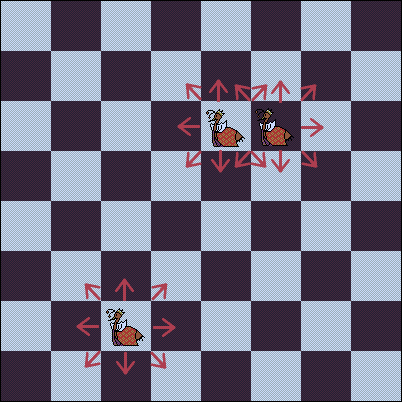
\includegraphics[width=0.60\linewidth]{possiveisMovimentacoes.png}
  \caption{Exemplo de possiveis movimentações de três rainhas no local search e na perturbação}
  \label{possiveisMovimentacoes}
\end{figure}

Pseudocódigo do ILS
\begin{algorithm}
  \KwData{rainhas, best, maxIterações}
  \KwResult{best - Melhor solução }
  $rainhas \gets randomStart(rainhas)$\;
  $rainhas \gets Local Search(rainhas)$\;
  $best \gets rainhas$\;
  \Repeat{$max Iterações$ OU $fitness(best)=1$}{
   $rainhas \gets perturbation(rainhas)$\;
   $rainhas \gets Local Search(rainhas)$\;
   \If{$fitness(rainhas)>fitness(best)$}{
     $best \gets rainhas$\;
   }
  }
  \label{pseudoILS}
  \caption{Pseudocódigo do algoritmo de ILS utilizado}
 \end{algorithm}

 \begin{algorithm}
  \KwData{population, best}
  \KwResult{best - Melhor fitness na população}
  $population \gets randomStart()$\;
  $populationFitness \gets fitness(population)$\;
  \Repeat{$maxIterações$ OU $\exists populationFitness=1$}{
   $population \gets algoritmoGenetico(population)$\;
   $populationFitness \gets fitness(population)$\;
  }
  $best \gets bestIn(population, populationFitness)$\;
  \caption{Pseudocódigo do Algoritmo Genético utilizado}
 \end{algorithm}
 

%%%%%%%%%%%%%%%%%%%%%%%%%%%%%%%%%%%%%%%%%%%%%%%%%%%%%%%%%%%%%%%%%%%%%%
\section{Resultados}

Nossos testes foram rodados em uma máquina Intel Core i5-7200U com 8GB de RAM, usando o sistema operacional Manjaro Linux com o pacote gráfico KDE Plasma. A linguagem de programação utilizada foi Python 3.7.1.

%%%%%%%%%%%%%%%%%%%%%%%%%%%%%%%%%%%%%%%%%%%%%%%%%%%%%%%%%%%%%%%%%%%%%%
\section{Conclusão}

Text...
\bookmarksetup{startatroot}% 
% ---

% ----------------------------------------------------------
% ELEMENTOS PÓS-TEXTUAIS
% ----------------------------------------------------------
\postextual

% ----------------------------------------------------------
% Referências bibliográficas
% ----------------------------------------------------------
%\bibliography{abnt}
\bibliography{bibliography}

\end{document}
